\title{Explore Weather Trends}
\author{Lucas Belpaire}

\documentclass{article}
\usepackage{listings}
\usepackage{graphicx}
\usepackage{subcaption}
\usepackage{float}
\begin{document}

\maketitle
\pagenumbering{gobble}

\newpage

\pagenumbering{arabic}

\section{Preparing data}

\subsection{Accessing Data With SQL}

The first step in this project is extracting the data out of the temperatures database using SQL statements.
\paragraph{}The following SQL statement extracts the attributes: year, city, country and average temperature of each record from the city\_data table. 
\begin{verbatim}
SELECT year, city, country, avg\_temp FROM city_data WHERE city='Brussels'
\end{verbatim}

The next SQL statement extracts the attributes: year, average temperature of each record from the global\_data table.
\begin{verbatim}
SELECT year, avg\_temp FROM global_data
\end{verbatim}

The data collected with these statements are stored as .csv files. We will use python to process these files.

\subsection{Python}

Organizing the data will be done by using Python. The NumPy library is used for calculations and the Matplotlib is used to plot the line graph. The libraries need to be imported which can be seen in the following python code.
\lstset{basicstyle=\footnotesize}
\begin{lstlisting}[language=Python]
import numpy as np 
import unicodecsv
import matplotlib.pyplot as plt
\end{lstlisting}

\paragraph{}
The first step is loading the data from the .csv files into variables we can use.
\begin{lstlisting}[language=Python]
def get_csv(filename):
    with open(filename, 'rb') as file:
        reader = unicodecsv.DictReader(file)
        return list(reader)

temperature_data_brussels = get_csv('belgiumTrends.csv')
temperature_data_global = get_csv('globalTrends.csv')
\end{lstlisting}

\paragraph{}
Because not all data is necessarily in the correct type, we will convert all data to the types we need.
\begin{lstlisting}[language=Python]
def correct_data_type(data):
	for data_entry in data:
		try:
		data_entry['avg_temp'] = float(data_entry['avg_temp'])
		except ValueError:
			data_entry['avg_temp'] = None
		try:
			data_entry['year'] = float(data_entry['year'])
		except ValueError:
			data_entry['year'] = None
	return data

corrected_data_brussels = correct_data_type(temperature_data_brussels)
corrected_data_global = correct_data_type(temperature_data_global)
\end{lstlisting}

\paragraph{}
The next step is calculating the moving average. The function 'get\_moving\_average' can calculate the moving average for different amount of years. In this example the amount is 10.
\begin{lstlisting}[language=Python]
def get_moving_average(data, length_of_average):
	
	last_n_years = np.zeros(length_of_average)

	for data_entry in data:
		temperature = data_entry['avg_temp']
		try:
			temperature = float(temperature)
			last_n_years = np.insert(last_n_years, 0, temperature)[:-1]
		except ValueError:
			last_n_years = np.insert(last_n_years, 0, 0)[:-1]
		except TypeError:
			last_n_years = np.insert(last_n_years, 0, 0)[:-1]
		if not 0 in last_n_years:
			data_entry['moving_average_temp'] = float(np.average(last_n_years))
		else:
			data_entry['moving_average_temp'] = None
	return data

temperature_moving_average_brussels = get_moving_average(corrected_data_brussels, 10)
temperature_moving_average_global = get_moving_average(corrected_data_global, 10)
\end{lstlisting}

\paragraph{}
After calculating all necessary values the line charts can be constructed. Which is done in the following code.
\begin{lstlisting}[language=Python]
def plot_graph(data, x_label, y_label, moving):
	years = []
	temperatures = []
	for data_entry in data:
		years.append(data_entry['year'])
		if moving:
			temperatures.append(data_entry['moving_average_temp'])
		else:
			temperatures.append(data_entry['avg_temp'])

	x = years
	y = temperatures
	plt.plot(x, y)
	plt.xlabel(x_label)
	plt.ylabel(y_label)
	plt.yticks(np.arange(5, 16, 1.0))
	plt.show()

plot_graph(temperature_moving_average_global, "Year", "Temperature (C°)", True)
plot_graph(temperature_moving_average_brussels, "Year", "Temperature (C°)", True)
\end{lstlisting}

\paragraph{Extra}
The function 'get\_temperatures' returns a NumPy list with all temperatures of a given list of data. This temperature list can be used by the function 'summarize\_data' to return the mean, standard deviation, minimum and maximum of that list of temperatures.
\begin{lstlisting}[language=Python]
def get_temperatures(data):
	temperatures = []
	for data_entry in data:
		try:
			temperatures.append(float(data_entry['avg_temp']))
		except:
			pass
	return np.array(temperatures)

def summarize_data(data):
	print ('Mean:', np.mean(data))
	print ('Standard deviation:', np.std(data))
	print ('Minimum:', np.min(data))
	print ('Maximum:', np.max(data))

summarize_data(get_temperatures(temperature_moving_average_global))
summarize_data(get_temperatures(temperature_moving_average_brussels))
\end{lstlisting}

To calculate the correlation coefficient the following method will be used.

\begin{lstlisting}
def correlation_coefficient(data):

	temperatures = []
	years = []

	for data_entry in data:
		try:
			temperature = float(data_entry['avg_temp'])
			year = float(data_entry['year'])
			temperatures.append(temperature)
			years.append(year)
		except:
			pass
	temperatures = np.array(temperatures)
	years = np.array(years)
	sum_temperatures = temperatures.sum()
	sum_years = years.sum()
	sum_years_times_temperatures = (years*temperatures).sum()
	sum_power_of_years = (years*years).sum()
	sum_power_of_temperatures = (temperatures*temperatures).sum()
	n = len(temperatures)

	return ((n * sum_years_times_temperatures) - (sum_temperatures * sum_years)) / 
		np.sqrt((n*sum_power_of_years - sum_years**2)*
		(n*sum_power_of_temperatures - sum_temperatures**2))

print(correlation_coefficient(temperature_moving_average_global))
print(correlation_coefficient(temperature_moving_average_brussels))

\end{lstlisting}

\section{Line Charts}
The following line charts are produces by the python code.

\begin{figure}[H]
\centering
\begin{subfigure}[h]{0.8\linewidth}
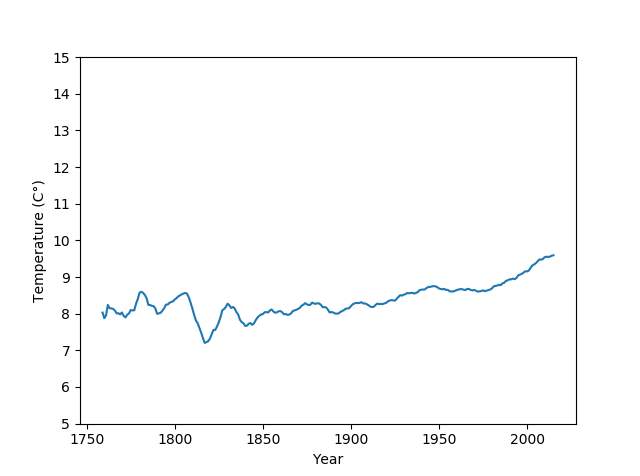
\includegraphics[width=\linewidth]{GlobalAverageTemperatureMoving.png}
\caption{Global Moving Average Temperature (10 years)}
\end{subfigure}
\begin{subfigure}[h]{0.8\linewidth}
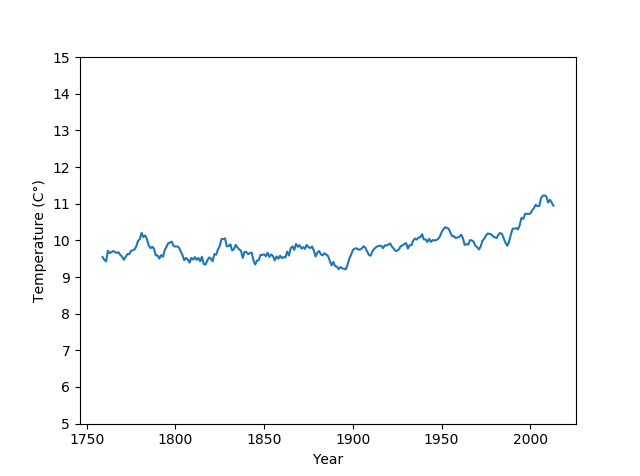
\includegraphics[width=\linewidth]{BrusselsAverageTemperatureMoving.png}
\caption{Brussels Moving Average Temperature (10 years)}
\end{subfigure}
\caption{Moving Average Temperature}
\label{fig:movingaveragetemp}
\end{figure}

\begin{figure}[H]
\centering
\begin{subfigure}[h]{0.9\linewidth}
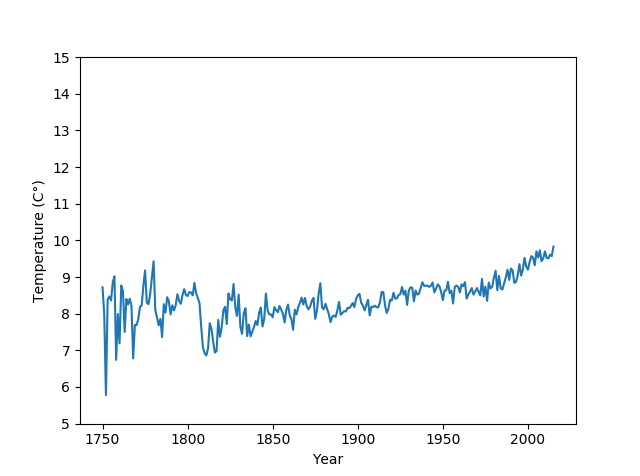
\includegraphics[width=\linewidth]{GlobalAverageTemperature.png}
\caption{Global Average Temperature}
\end{subfigure}
\begin{subfigure}[h]{0.9\linewidth}
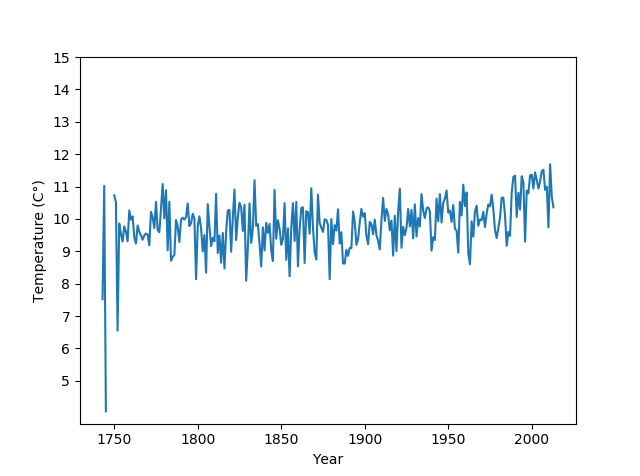
\includegraphics[width=\linewidth]{BrusselsAverageTemperature.png}
\caption{Brussels Average Temperature}
\end{subfigure}
\caption{Average Temperature}
\label{fig:averagetemp}
\end{figure}

\section{Observations}

Executing the summarize\_data function and correlation\_coefficient function results in the following values:

\begin{verbatim}
Global temperature:
Mean: 8.369473684210526
Standard deviation: 0.5836472255514844
Minimum: 5.78
Maximum: 9.83
Correlation coefficient: 0.6227745062665663

Brussels temperature:
Mean: 9.85059925093633
Standard deviation: 0.8252501700366419
Minimum: 4.06
Maximum: 11.69
Correlation coefficient: 0.3821422210006082
\end{verbatim}


It is easy to conclude that the mean temperature in Brussels is higher than the global mean. The minimum temperature of Brussels is also lower than the global minimum, the highest temperature of Brussel is also higher than the global highest temperature. 

That the difference in minimum and maximum temperature in Brussel is more extreme than the difference between global minimum and maximum can also be seen by Brussels' standard deviation, which is higher than the global one.

\paragraph{}
The correlation coefficient of the global average graph is 0.62. This means there is a positive correlation between year and temperature. Meaning the temperature will rise as the years increase.
The correlation coefficient of the Brussels average graph is 0.38. which also means a positive correlation between year and temperature. The coefficient is lower than the coefficient of the global average, which means that the temperature will also rise as the years increase, but less quickly.

\paragraph{}
When looking at figure 1.a and figure 1.b it is clear that the average temperature is higher in Brussels than globally. This also corresponds with the higher mean temperature in Brussels compared to the global mean temperature.

\paragraph{}
Overall figure 1.a is a lot smoother than figure 1.b. The most probable reason is that the global temperature will not be affected by local outliers, which can be the case in a city like Brussels. 

\paragraph{}
Comparing figure 1 and figure 2 clearly  shows the difference between a moving average and an average. The line charts in figure 2 are a lot less smooth than the ones in figure 1. It is a lot harder to read trends in figure 2 which is why a moving average can be very effective.
































\end{document}